% ----------------------------------------------------
% -------- BAYSIS - Selected as Jam Follower ---------
% ----------------------------------------------------
\subsection{BAYSIS - Selected as Jam Follower}
\label{analysis_processing_correlation_baysis_follower}
The correlation matrix table for the congestion-accident \textit{Jam Follower} dataset (see \cref{table:appendix_correlation_matrix_matched_cramers}) is visual presented in \cref{img:correlation_matrix_selected_effector_cramers} showing the the correlation of each variable combination. When visual analyzing \cref{img:correlation_matrix_matched_cramers} and checking the guidelines for a strong correlation in reference to the applied coefficient (identifiable with \cref{table:appendix_coefficient_matrix_matched}) we get a list of strongly correlated variable combinations (see \cref{tbl:correlation_list_baysis_follower})

\noindent
\begin{table}[h!]
	\centering
	\begin{tabular}{c|l}  
		Category & Strong \\
		\\[-1em]
		\hline
		\\[-1em]
		Strasse & TMax, TAvg, SMax, SAvg, TDist, SDist, Cov, TLHGV \\ 
 		Kat & TMax, SAvg\\ 
 		%Typ & \\
 		%Betei & \\
 		UArt1 & TAvg, SAvg, TDist, Cov, TLHVG \\
 		UArt2 & TDist \\
 		AUrs1 & TDist, SDist, Cov, TLHGV \\
 		%AUrs2 & \\
 		AufHi & TMax, TAvg, Cov \\
 		%Alkoh & \\
 		%Char1 & \\
 		%Char2 & \\
 		%Bes1 & \\
 		%Bes2 & \\
 		Lich1 & Cov \\
 		%Lich2 & \\
 		%Zust1 & \\
 		%Zust2 & \\
 		%Fstf & \\
 		WoTag & TAvg, SMax, SAvg, TDist, Cov, TLHGV \\
 		%FeiTag & \\
 		Month & TMax, TAvg, SMax, Cov, TLHGV \\
	\end{tabular}
    \caption{List of incident variables and their strong correlated congestion variable from the congestion-accident matched data which are classified as \textit{Jam Follower}}
	\label{tbl:correlation_list_baysis_follower}
\end{table}

Next we need to verify that the correlation is significant and what the correlation predicates. Therefore each correlation will be evaluated with the Post Hoc test, defined in \cref{correlation_posthoc}. In the following sections, the correlated relations of the variables in \cref{tbl:correlation_list_baysis_follower} are analyzed and an initial interpretation of each significant correlation is introduced. Groups with an insufficient sample size (see \cref{correlation_uncertainty} are neglected and not shown. The descriptive tables, showing the count ($n$), mean ($\bar{x}$), standard deviation ($\sigma$), median ($\tilde{x}$), $min$, $max$ and range ($\Delta$) therefore only contain groups with significant sample sizes.

\begin{figure}[!ht]
	\centering
	\makebox[\textwidth][c]{%
		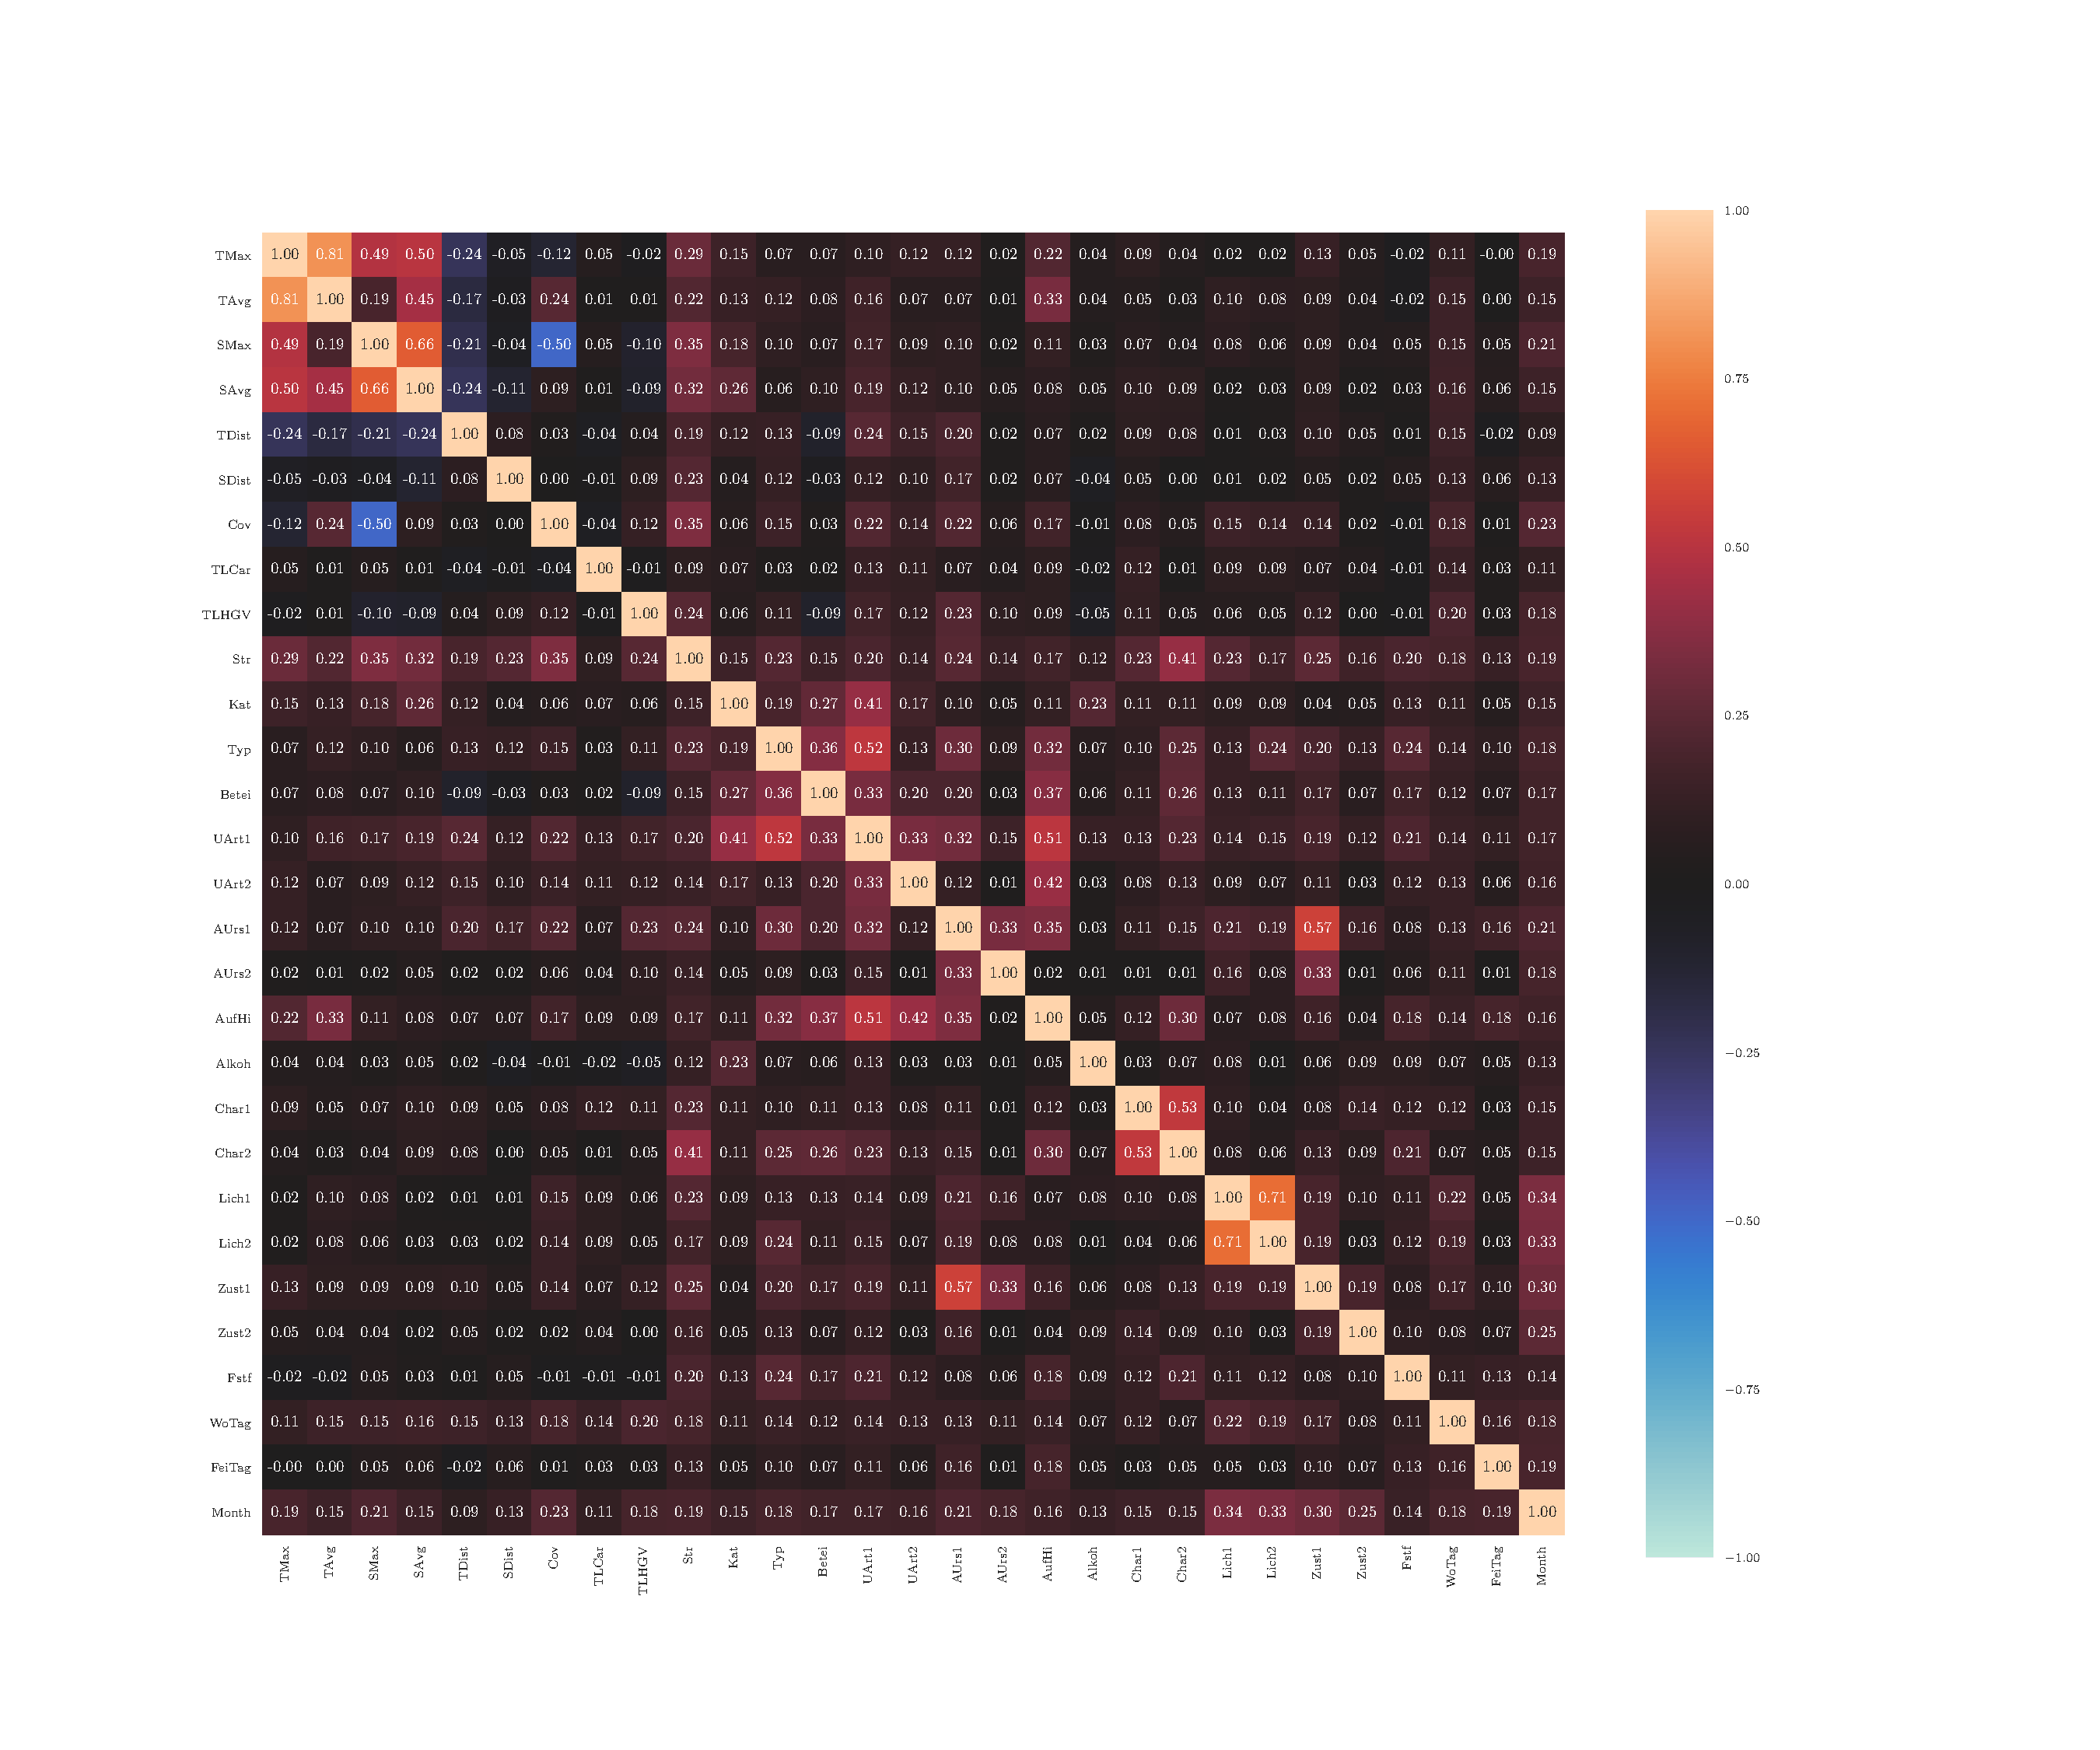
\includegraphics[width=1.4\textwidth, trim=0cm 2.5cm 6cm 3cm]{CorrAnalysis/data/BAYSIS/03_selected_03_endJam/plots/baysis_selected_corr_cramers}%
	}
	\caption{Correlation matrix for congestion-accident matched data classified as \textit{Jam Effector}, with $V$, $\eta$, $\tau$, $r_{pq}$, $r$}
	\label{img:correlation_matrix_selected_effector_cramers}
\end{figure}

% --------------------------
% -------- Strasse ---------
% --------------------------
\centerheading{Strasse}
All relations of \textit{Strasse} - \textit{TMax}, \textit{Strasse} - \textit{TAvg}, \textit{Strasse} - \textit{SMax}, \textit{Strasse} - \textit{SAvg}, \textit{Strasse} - \textit{TDist}, \textit{Strasse} - \textit{SDist}, \textit{Strasse} - \textit{Cov} and \textit{Strasse} - \textit{TLHGV} produce a $p$-value above the $\alpha$-level. The null hypothesizes can't be rejected and there are \textit{no} significant differences between the groups of \textit{Strasse} in these relations.

% ----------------------
% -------- Kat ---------
% ----------------------
\centerheading{Kat}
Both relations of \textit{Kat} - \textit{TMax} and \textit{Kat} - \textit{SAvg} produce a $p$-value above the $\alpha$-level. The null hypothesizes can't be rejected and there are \textit{no} significant differences between the groups of \textit{Kat} in these relations.

% ------------------------
% -------- UArt ---------
% ------------------------
\centerheading{UArt1}
All relations of \textit{UArt1} - \textit{TAvg}, \textit{UArt1} - \textit{SAvg}, \textit{UArt1} - \textit{TDist}, \textit{UArt1} - \textit{Cov}, \textit{UArt1} - \textit{TLHGV} and \textit{UArt2} - \textit{TDist} produce a $p$-value above the $\alpha$-level. The null hypothesizes can't be rejected and there are \textit{no} significant differences between the groups of \textit{Strasse} in these relations.

% ------------------------
% -------- AUrs ---------
% ------------------------
\centerheading{AUrs1}

\paragraph{Temporal Distance}
Kruskal-Wallis chi-squared = 15.692, df = 24, p-value = 0.8989

\paragraph{Time-loss HGV}
Kruskal-Wallis chi-squared = 313.02, df = 293, p-value = 0.2015

\paragraph{Spatial Distance}
Kruskal-Wallis chi-squared = 104.3, df = 79, p-value = 0.0299

\begin{table}[ht]
	\tiny
	\centering
	\begin{tabular}{rrrrrrr}
		\hline
		& 0 & 72 & 73 & 80 & 82 & 88 \\ 
		\hline
		72 & 1.00 &  &  &  &  &  \\ 
		73 & 0.09 & 0.35 &  &  &  &  \\ 
		80 & 1.00 &  & 1.00 &  &  &  \\ 
		82 & 1.00 &  & 1.00 &  &  &  \\ 
		88 & 0.36 & 0.04 & 1.00 & 1.00 & 0.55 &  \\ 
		89 & 1.00 &  & 1.00 &  &  & 1.00 \\ 
		\hline
	  \end{tabular}
    \caption{Pairwise Wilcoxon $T$-test for \textit{AUrs1} and \textit{Spatial Distance} (Jam Follower)}
    \label{tbl:wilcoxon_baysis_follower_AUrs1_SDist}
\end{table}
\todo{Explain}
\begin{table}[ht]
	\tiny
	\centering
	\begin{tabular}{rrrrrrrrrrrrrr}
		\hline
		& vars & n & mean & sd & median & trimmed & mad & min & max & range & skew & kurtosis & se \\ 
		\hline
		X1 & 1.00 & 437.00 & 100.42 & 294.15 & 0.00 & 19.26 & 0.00 & 0.00 & 1949.00 & 1949.00 & 3.77 & 15.04 & 14.07 \\ 
		X11 & 1.00 & 9.00 & 0.00 & 0.00 & 0.00 & 0.00 & 0.00 & 0.00 & 0.00 & 0.00 &  &  & 0.00 \\ 
		X12 & 1.00 & 16.00 & 369.00 & 583.01 & 0.00 & 278.86 & 0.00 & 0.00 & 2000.00 & 2000.00 & 1.50 & 1.30 & 145.75 \\ 
		X13 & 1.00 & 1.00 & 0.00 &  & 0.00 & 0.00 & 0.00 & 0.00 & 0.00 & 0.00 &  &  &  \\ 
		X14 & 1.00 & 4.00 & 0.00 & 0.00 & 0.00 & 0.00 & 0.00 & 0.00 & 0.00 & 0.00 &  &  & 0.00 \\ 
		X15 & 1.00 & 2.00 & 3.00 & 0.00 & 3.00 & 3.00 & 0.00 & 3.00 & 3.00 & 0.00 &  &  & 0.00 \\ 
		X16 & 1.00 & 2.00 & 0.00 & 0.00 & 0.00 & 0.00 & 0.00 & 0.00 & 0.00 & 0.00 &  &  & 0.00 \\ 
		\hline
	  \end{tabular}
    \caption{Group descriptives of \textit{AUrs1} and \textit{Spatial Distance} (Jam Follower)}
    \label{tbl:descriptives_baysis_follower_AUrs1_SDist}
	%\vspace{-8mm}
\end{table}

\paragraph{Coverage}
Kruskal-Wallis chi-squared = 114.97, df = 77, p-value = 0.003296

\begin{table}[ht]
	\tiny
	\centering
	\begin{tabular}{rrrrrrr}
		\hline
		& 0 & 72 & 73 & 80 & 82 & 88 \\ 
		\hline
		72 & 0.28 &  &  &  &  &  \\ 
		73 & 1.00 & 1.00 &  &  &  &  \\ 
		80 & 1.00 & 1.00 & 1.00 &  &  &  \\ 
		82 & 1.00 & 1.00 & 1.00 & 1.00 &  &  \\ 
		88 & 0.33 & 0.79 & 0.56 & 1.00 & 1.00 &  \\ 
		89 & 1.00 & 1.00 & 1.00 & 1.00 & 1.00 & 1.00 \\ 
		\hline
	  \end{tabular}
    \caption{Pairwise Wilcoxon $T$-test for \textit{AUrs1} and \textit{Coverage} (Jam Follower)}
    \label{tbl:wilcoxon_baysis_follower_AUrs1_Cov}
\end{table}
\todo{Explain}
\begin{table}[ht]
	\tiny
	\centering
	\begin{tabular}{rrrrrrrrrrrrrr}
		\hline
		& vars & n & mean & sd & median & trimmed & mad & min & max & range & skew & kurtosis & se \\ 
		\hline
		X1 & 1.00 & 437.00 & 36.35 & 18.02 & 35.00 & 35.12 & 17.79 & 2.00 & 100.00 & 98.00 & 0.66 & 0.32 & 0.86 \\ 
		X11 & 1.00 & 9.00 & 50.22 & 13.94 & 49.00 & 50.22 & 16.31 & 28.00 & 67.00 & 39.00 & -0.20 & -1.65 & 4.65 \\ 
		X12 & 1.00 & 16.00 & 41.44 & 18.39 & 39.50 & 41.79 & 25.20 & 10.00 & 68.00 & 58.00 & -0.14 & -1.35 & 4.60 \\ 
		X13 & 1.00 & 1.00 & 48.00 &  & 48.00 & 48.00 & 0.00 & 48.00 & 48.00 & 0.00 &  &  &  \\ 
		X14 & 1.00 & 4.00 & 35.50 & 22.04 & 28.50 & 35.50 & 11.86 & 18.00 & 67.00 & 49.00 & 0.56 & -1.83 & 11.02 \\ 
		X15 & 1.00 & 2.00 & 88.00 & 0.00 & 88.00 & 88.00 & 0.00 & 88.00 & 88.00 & 0.00 &  &  & 0.00 \\ 
		X16 & 1.00 & 2.00 & 37.00 & 11.31 & 37.00 & 37.00 & 11.86 & 29.00 & 45.00 & 16.00 & 0.00 & -2.75 & 8.00 \\ 
		\hline
	  \end{tabular}
    \caption{Group descriptives of \textit{AUrs1} and \textit{Coverage}}
    \label{tbl:descriptives_baysis_follower_AUrs1_Cov}
	%\vspace{-8mm}
\end{table}

\paragraph{Time-loss HGV}
Kruskal-Wallis chi-squared = 313.02, df = 293, p-value = 0.2015

\large
\centerline{\textbf{AufHi}}
\normalsize

\paragraph{Maximal temporal Extent:}
Kruskal-Wallis chi-squared = 154.9, df = 168, p-value = 0.7572

\paragraph{Average temporal Extent:}
Kruskal-Wallis chi-squared = 157.26, df = 173, p-value = 0.7987

\paragraph{Coverage}
Kruskal-Wallis chi-squared = 93.325, df = 77, p-value = 0.09933

\large
\centerline{\textbf{Lich1}}
\normalsize

\paragraph{Coverage}
Kruskal-Wallis chi-squared = 88.003, df = 77, p-value = 0.1839

\large
\centerline{\textbf{WoTag}}
\normalsize

\paragraph{Maximal temporal Extent:}
Kruskal-Wallis chi-squared = 168.61, df = 167, p-value = 0.4506

\paragraph{Maximal spatial Extent:}
Kruskal-Wallis chi-squared = 448.61, df = 425, p-value = 0.2067

\paragraph{Average spatial Extent:}
Kruskal-Wallis chi-squared = 460.72, df = 433, p-value = 0.1723

\paragraph{Temporal Distance}
Kruskal-Wallis chi-squared = 22.628, df = 24, p-value = 0.5418

\paragraph{Coverage}
Kruskal-Wallis chi-squared = 73.906, df = 77, p-value = 0.5788

\paragraph{Time-loss HGV}
Kruskal-Wallis chi-squared = 318.99, df = 293, p-value = 0.1422

\large
\centerline{\textbf{Month}}
\normalsize

\paragraph{Maximal temporal Extent:}
Kruskal-Wallis chi-squared = 165.89, df = 168, p-value = 0.5316

\paragraph{Average temporal Extent:}
Kruskal-Wallis chi-squared = 182.94, df = 173, p-value = 0.2877

\paragraph{Maximal spatial Extent:}
Kruskal-Wallis chi-squared = 460.69, df = 427, p-value = 0.1258

\paragraph{Coverage}
Kruskal-Wallis chi-squared = 70.545, df = 77, p-value = 0.6849

\paragraph{Time-loss HGV}
Kruskal-Wallis chi-squared = 293.39, df = 293, p-value = 0.4826